%%PREAMBLE %%%%%%%%%%%%%%%%%%%%%%%%%%%%
\documentclass[10pt, a4paper]{article}% size of txt = 10pt
\usepackage[top= 2cm,
			bottom = 2cm,
			left = 1.7cm,
			right = 1.7cm,
			footskip = 0.5cm,
			headsep = 0cm,
			headheight = 0cm
					]{geometry}
\usepackage{amsmath} % math packages
\usepackage{amsfonts}% math packages
\usepackage{amssymb} % math packages
\usepackage{graphicx} %package for including graphics
\usepackage{array}
\usepackage[thinlines]{easytable}
\usepackage{float}
\usepackage[section]{placeins}
\usepackage[hidelinks]{hyperref}
\usepackage[shortlabels]{enumitem}
\usepackage{svg}
\usepackage{bigstrut}
\usepackage{wrapfig,lipsum,booktabs}
\usepackage{subcaption}
\usepackage{xfrac}
\usepackage{pdfpages}
\usepackage{listings}
\usepackage{xcolor}


\usepackage{listings}
\usepackage{color} %red, green, blue, yellow, cyan, magenta, black, white
\definecolor{mygreen}{RGB}{28,172,0} % color values Red, Green, Blue
\definecolor{mylilas}{RGB}{170,55,241}

\definecolor{codegreen}{rgb}{0,0.6,0}
\definecolor{codegray}{rgb}{0.5,0.5,0.5}
\definecolor{codepurple}{rgb}{0.58,0,0.82}
\definecolor{backcolour}{rgb}{1,1,1}

\lstdefinestyle{mystyle}{
    backgroundcolor=\color{backcolour},   
    commentstyle=\color{codegreen},
    keywordstyle=\color{magenta},
    numberstyle=\tiny\color{codegray},
    stringstyle=\color{codepurple},
    basicstyle=\ttfamily\footnotesize,
    breakatwhitespace=false,         
    breaklines=true,                 
    captionpos=b,                    
    keepspaces=true,                 
    numbers=left,                    
    numbersep=5pt,                  
    showspaces=false,                
    showstringspaces=false,
    showtabs=false,                  
    tabsize=2
}
\lstset{style=mystyle}


%date format
\def\mydate{\leavevmode\hbox{\twodigits\day.\twodigits\month.\the\year}}
\def\twodigits#1{\ifnum#1<10 0\fi\the#1}

\usepackage{indentfirst}
\setlength{\parindent}{1cm}

\makeatletter
\newcommand{\thickhline}{%
    \noalign {\ifnum 0=`}\fi \hrule height 2pt
    \futurelet \reserved@a \@xhline
}
\newcolumntype{"}{@{\hskip\tabcolsep\vrule width 2pt\hskip\tabcolsep}}
\makeatother
\newcolumntype{?}{!{\vrule width 2pt}}
%%DOC ENVIROMENT%%%%%%%%%%%%%%%%%%%%%%%xx
\begin{document}
%Title 
\begin{flushleft}%% left justification
	\textbf{\Large{MKC-IKS: Úkol č. 2}}\hfill Filip Paul\\
	\large{Časová synchronizace OFDM a odhad CFO \hfill\mydate}
\end{flushleft}
	\section*{\Large Úkol 1 - Synchronizace:}
        \subsection*{Korelace lokální repliky}
        Na obrázku níže je patrných 8 korelačních špiček, to je způsobeno tím, že preambule má délku $8\cdot 16$ symbolů, přičemž
        lokální replika má délku 16 symbolů. Problémem této metody je, že koreluje signál zkreslený průchodem kanálu ze
        signálem bez zkreslení. To v případě zašumělého kanálu může zhoršit korelační vlastnosti.

        \subsection*{Schmidl a Cox:}
        Metoda Schmidl a Cox, koreluje přijaté části signálů mezi sebou. Vzhledem k tomu, že všechny korelované části signálů
        prochází kanálem v krátkém časovém úseku mají mezi sebou lepší korelační vlastnosti než v případě metody pomocí
        lokální repliky.
        Nevýhodou této motody je, že vzniká v časové oblasti "plato" a nelze tak jednoznačně určit čas synchronizace.
        Pro jednoznačné určení, je potřeba zavést detekci sestupné hrany s tresholdem takovým, aby setupná hrana byla zachycena
        po ukončení oblasti s "platem".

        \subsection*{Schmidl a Cox:}
        Problém metody Schmidl a Cox řeší metoda WANG. Zde vzniká po korelaci špička a synchronizace je tak určena v bodě (čase)
        s nejvyšší korelací.

        \begin{figure}[ht!]
            \centering
            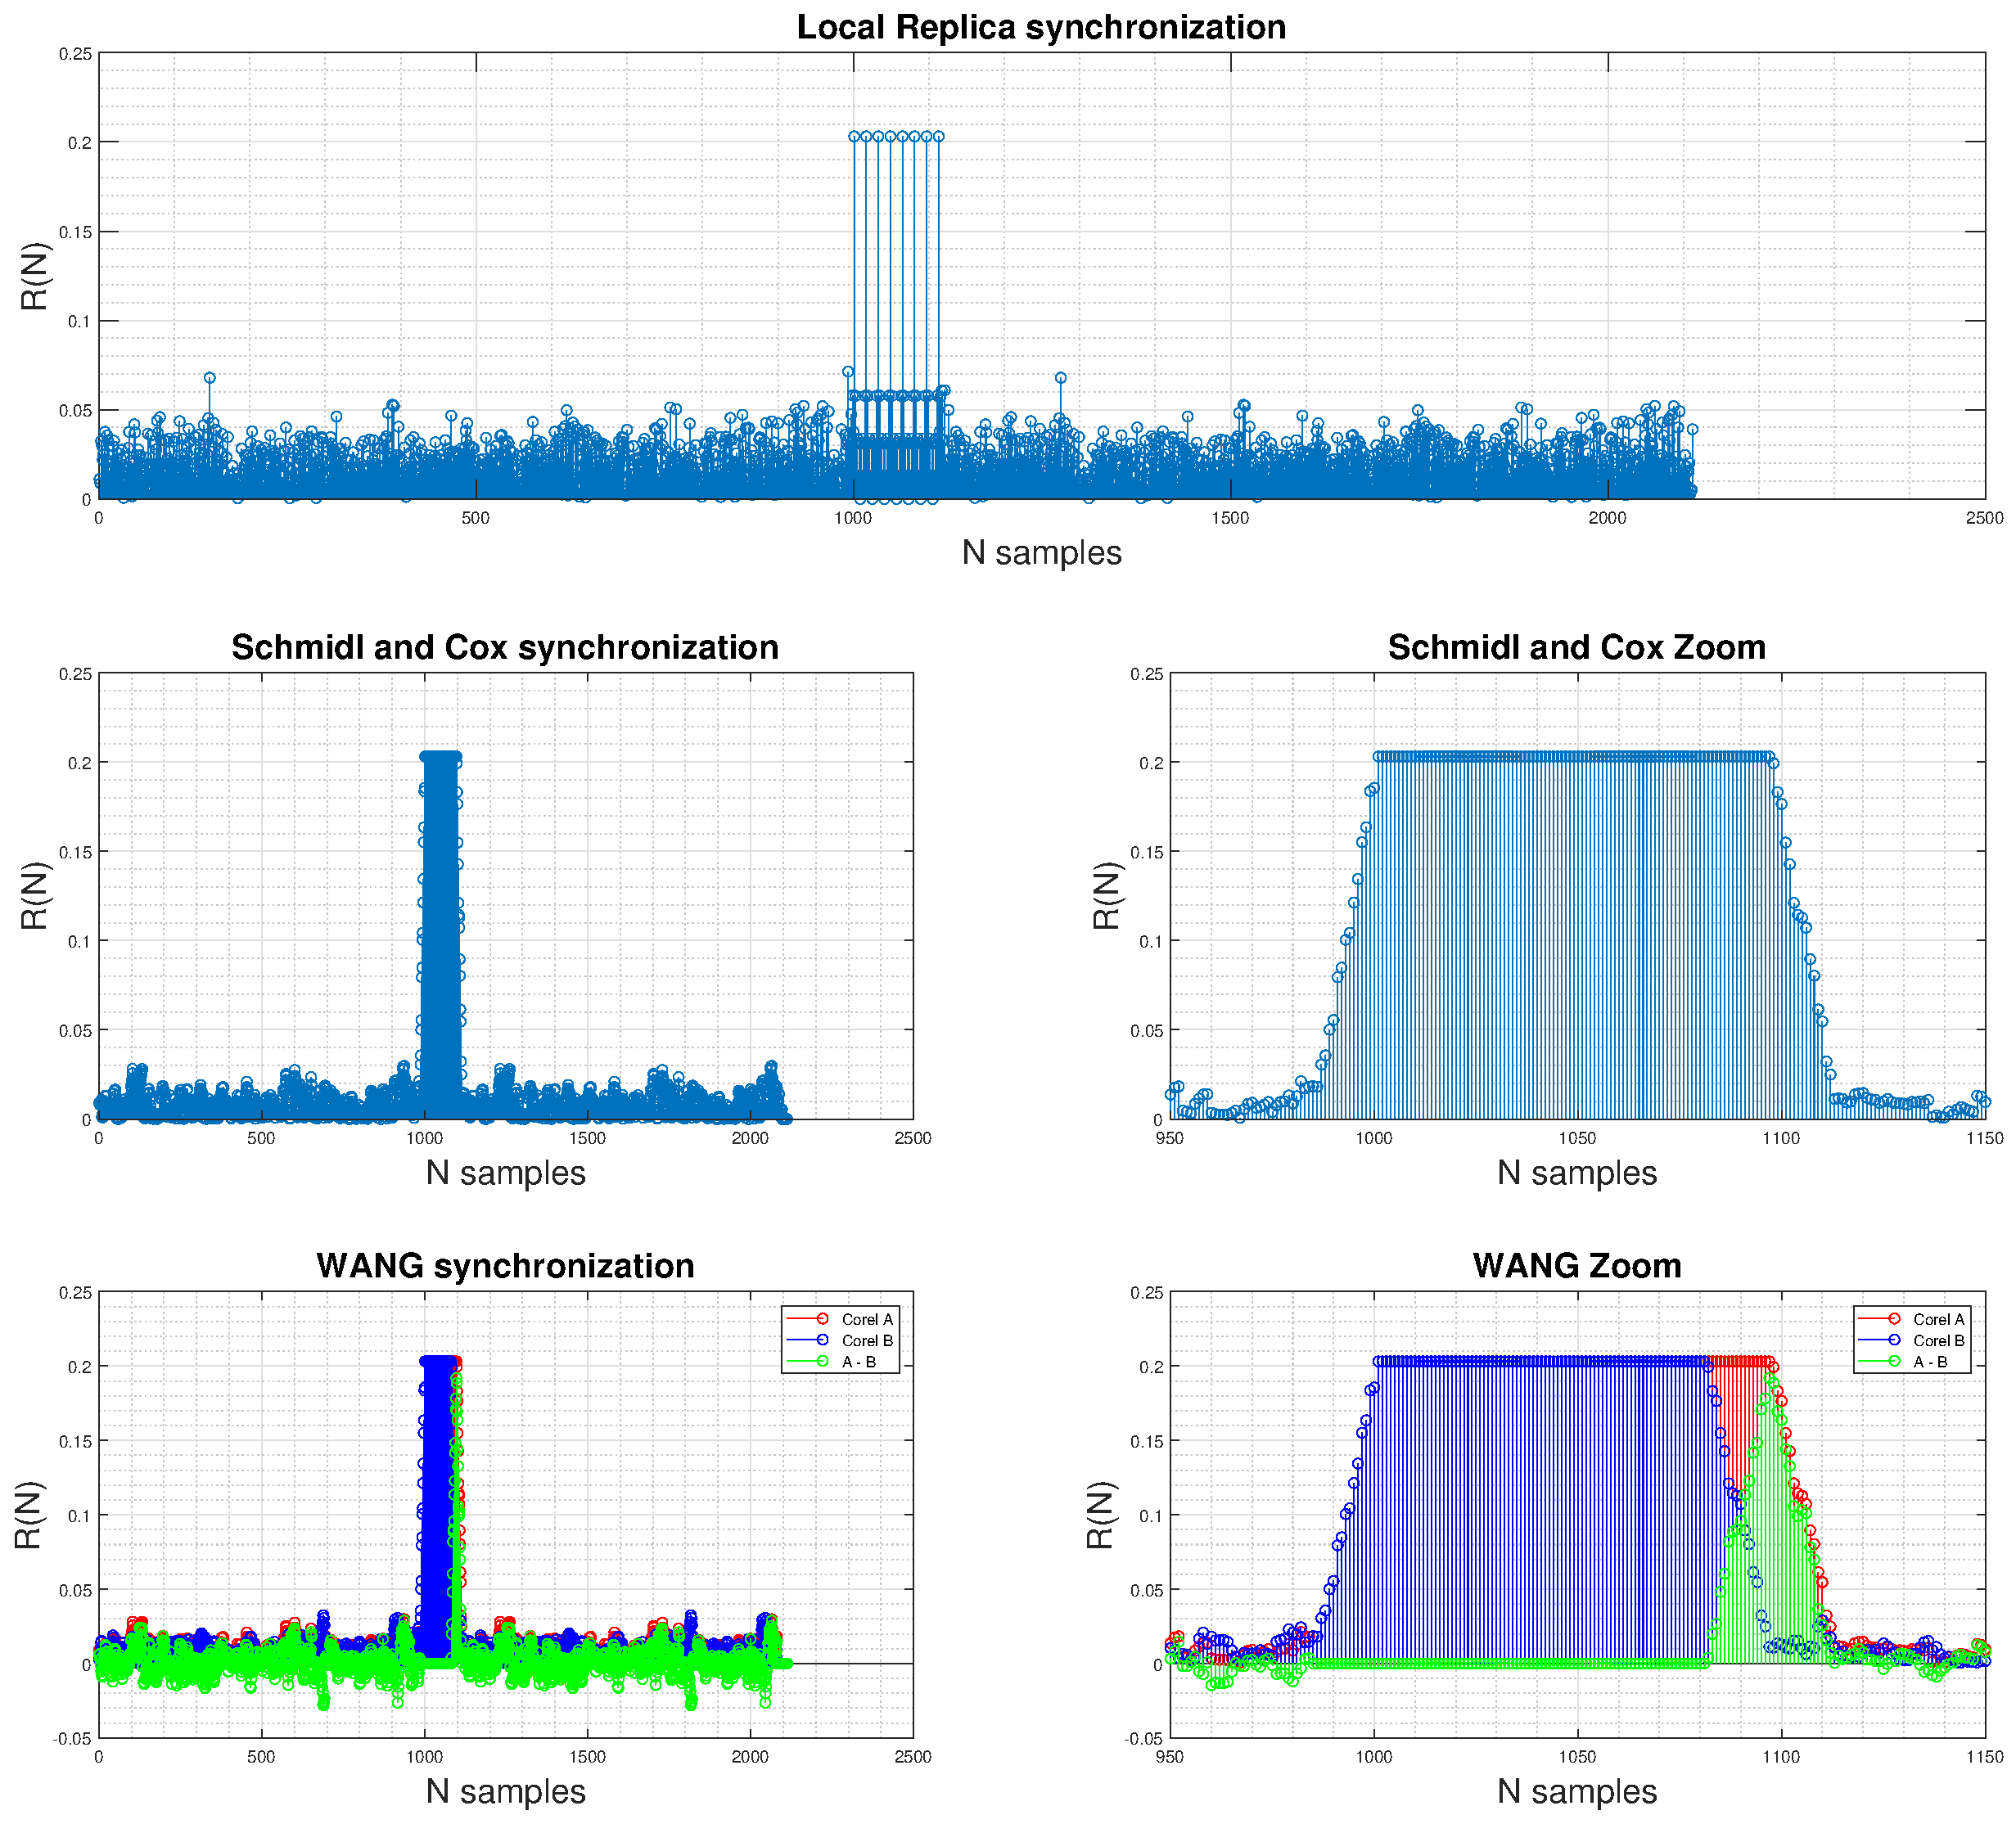
\includegraphics[width = 0.95\textwidth]{cviceni/sync.eps}
        \end{figure}

	\clearpage
	\section*{\Large Úkol 2 - synchronizace s CFO:}

    \begin{figure}[ht!]
        \centering
        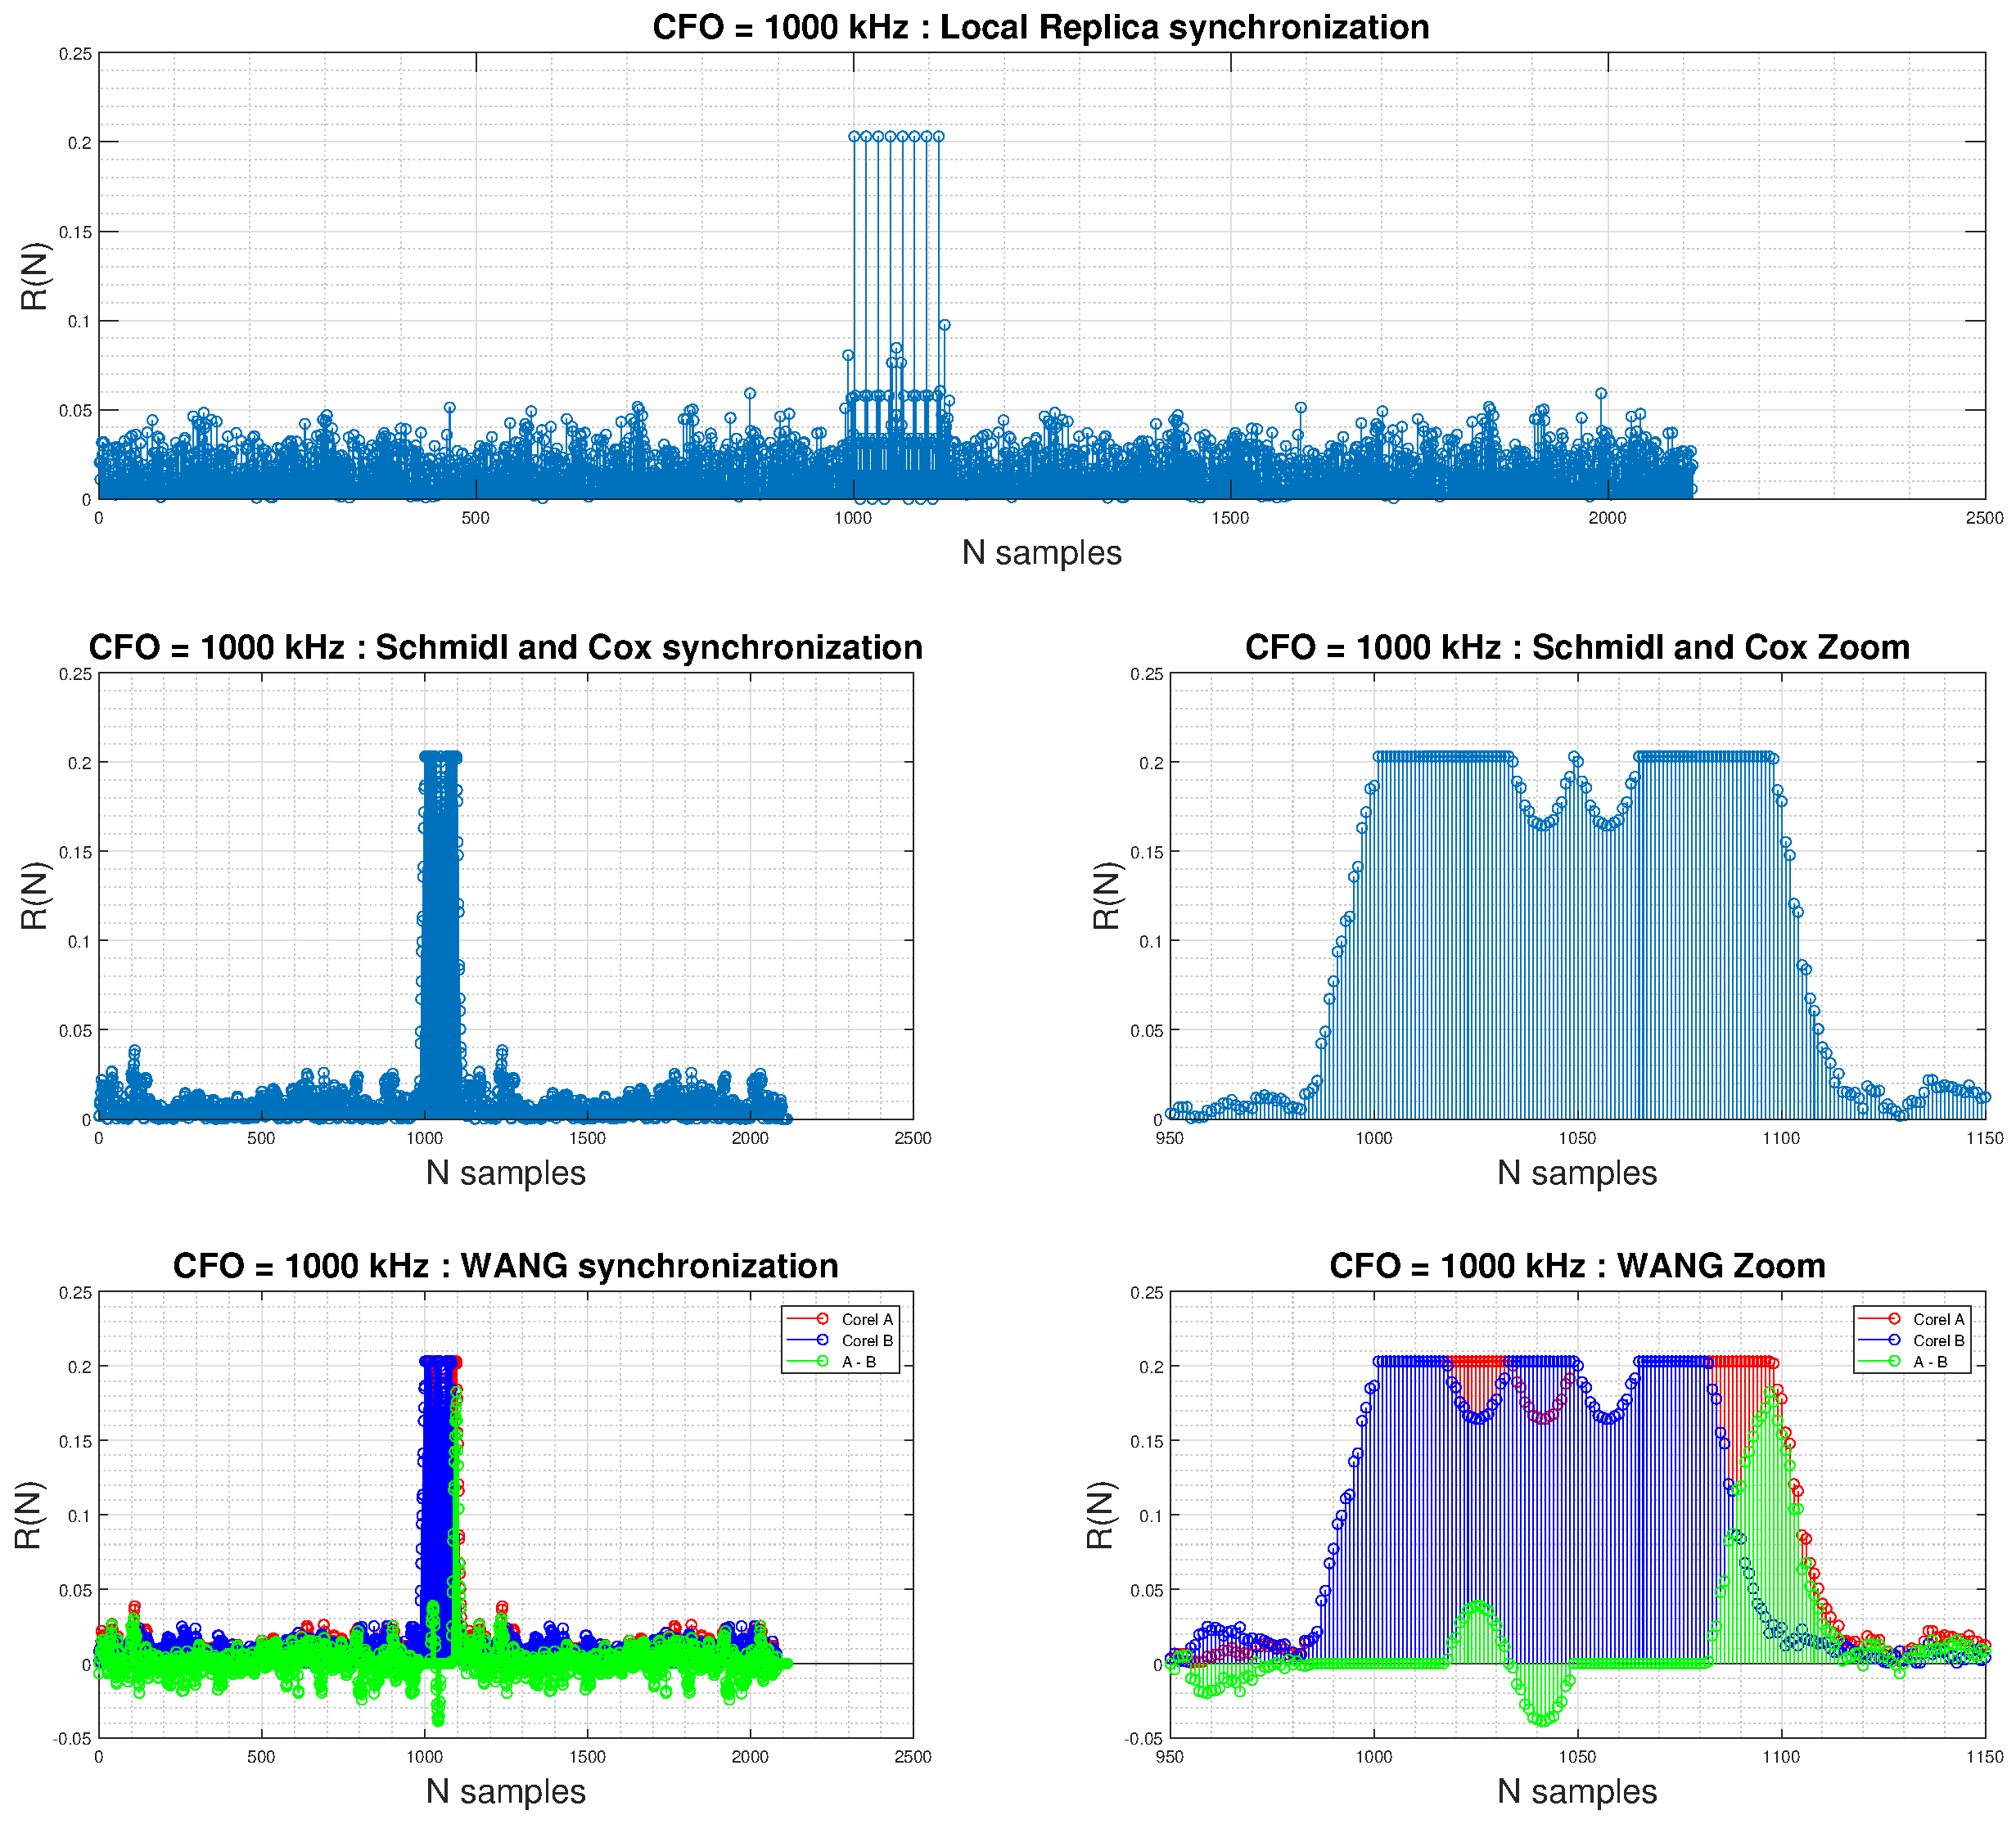
\includegraphics[width = 0.95\textwidth]{cviceni/sync_CFO.eps}
    \end{figure}

    \section*{\Large Úkol 3 - Odhad CFO:}
    Na následujících obrázcích je znázorněn odhat CFO pomocí metody MOOSE. Při simulaci se projevuje i přenosový kanál, který
    není stejný pro oba zobrazené SNR. Z obrázků je patrné, že při horším SNR se zhorší i odhad CFO, kde dokonce pro některé
    vzorky má opačné znaménko než by se očekávalo.

    \begin{figure}[ht!]
        \centering
        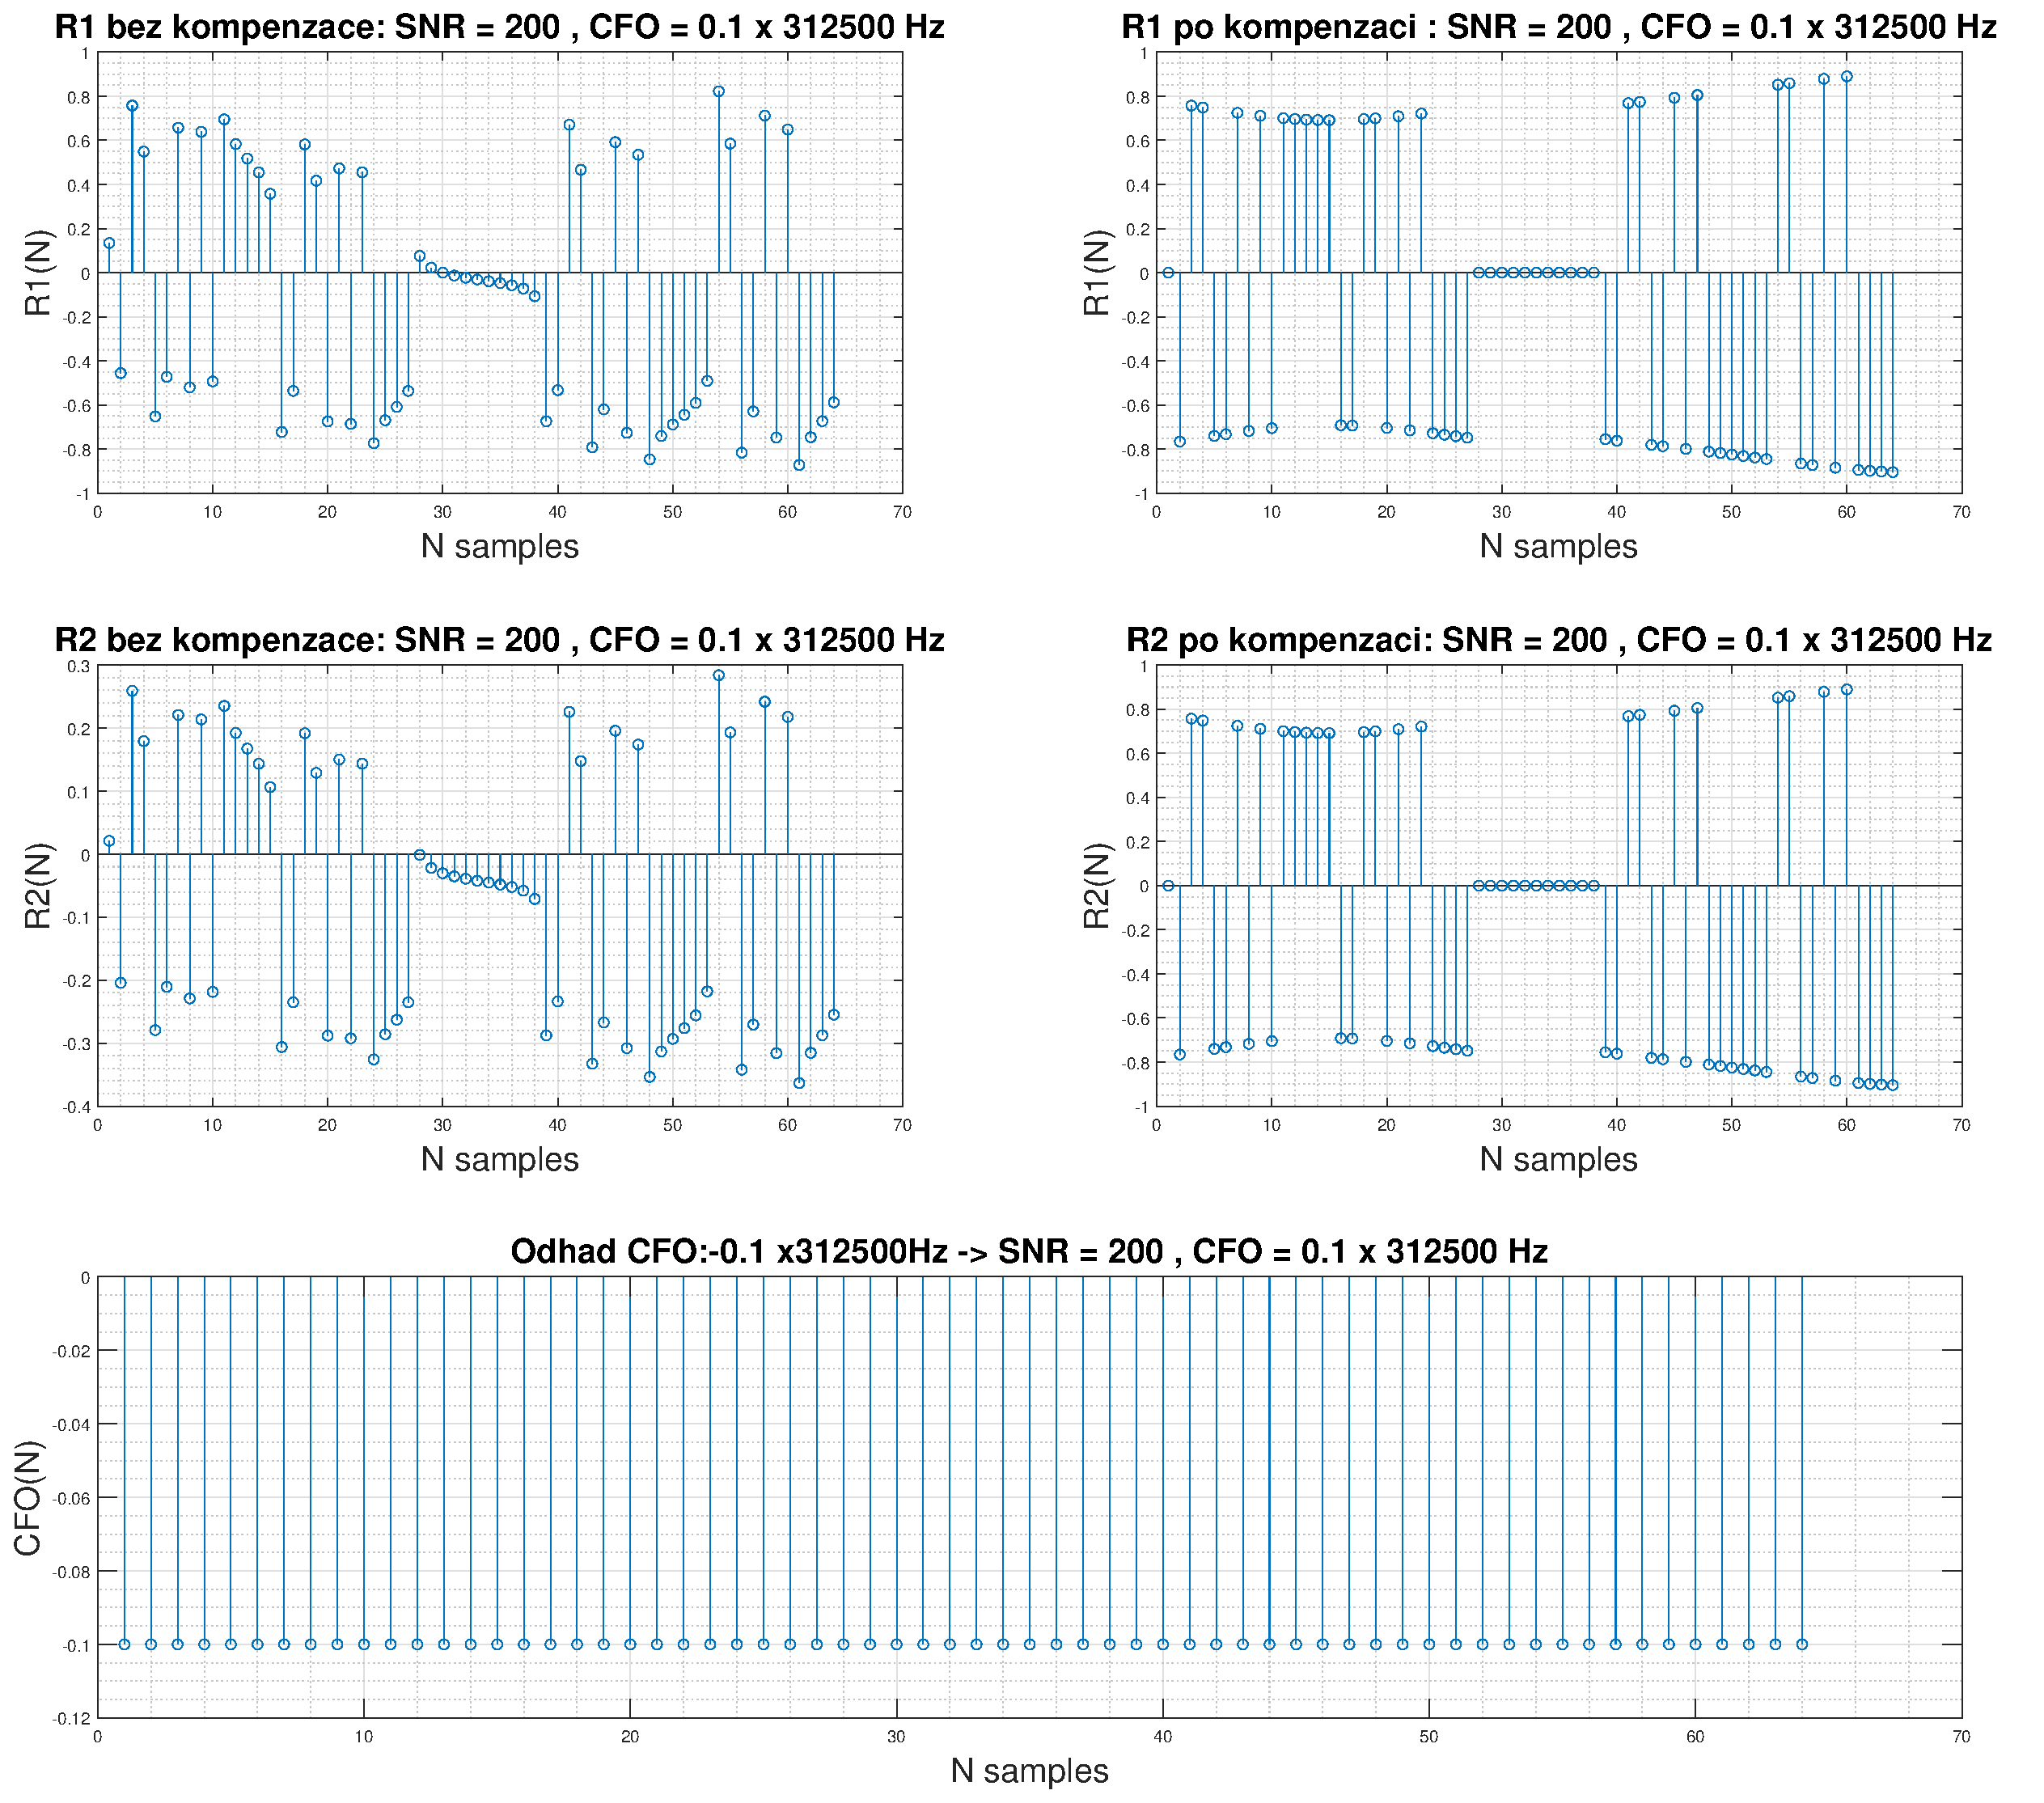
\includegraphics[height = 0.45\textheight]{cviceni/SNR_200.eps}
    \end{figure}

    \begin{figure}[ht!]
        \centering
        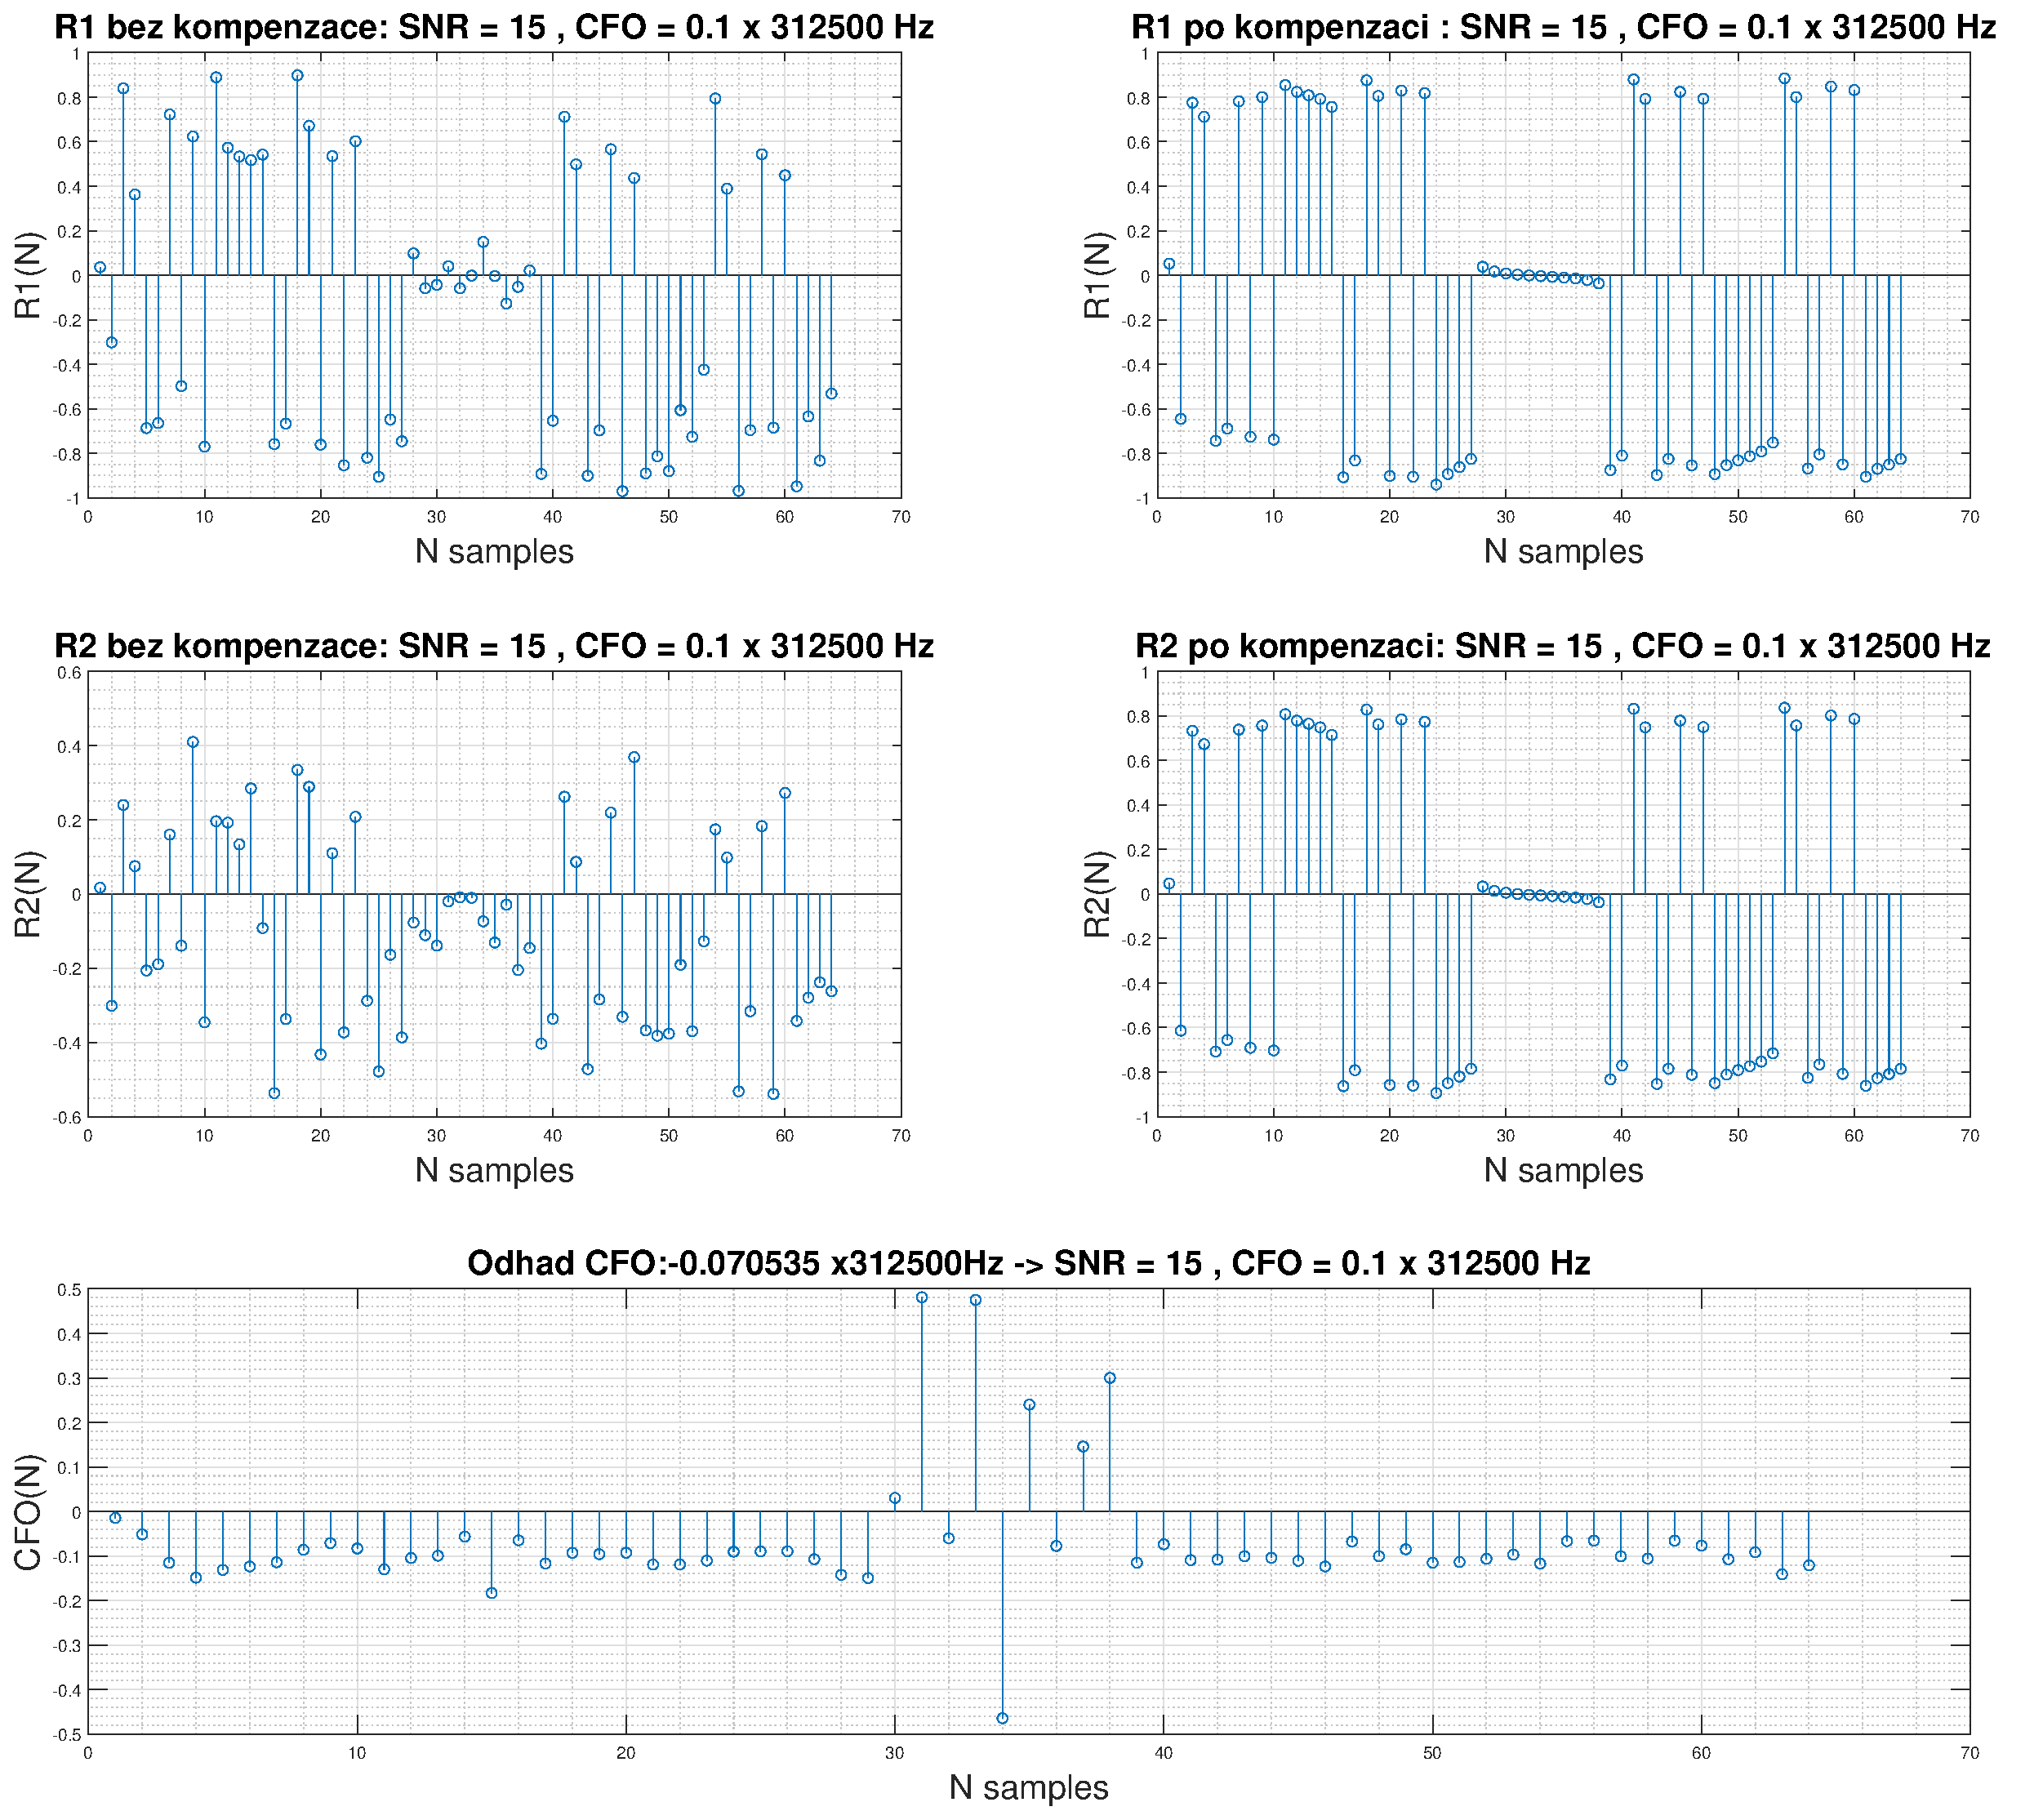
\includegraphics[height = 0.45\textheight]{cviceni/SNR_15.eps}
    \end{figure}
    \clearpage
\section*{\Large Přílohy:}
Všechny MATLAB scripty si můžete zobrazit/stáhnout i v mojem github
repozitáři \href{https://github.com/FilipPaul/ctvrtak_letni_semestr/blob/main/MKC_IKS/ukol_2_OFDM_CFO/README.md}{\color{blue} zde}.
\subsection*{IKS\_synchroniz\_empty.m}
\lstinputlisting[language=matlab]{cviceni/IKS_synchroniz_empty.m}
\clearpage
\subsection*{MIKS\_CFOest\_student.m}
\lstinputlisting[language=matlab]{cviceni/MIKS__CFOest_student.m}

\end{document}
%\[f(x)= (x+2)^2 - \frac{9\cdot 2\pi}{26}\] %%mathematic equatation in display style mode
%%optional:
%	\begin{align} %%this alignes all charakters after & if *is removed equations will be numbered
%	\hspace{5cm}  
%		 x &= a_2 x^2 +_1 x + a_0 \\
% 		x &=x^2 \nonumber		%no number will not add number to eq
%	\end{align}